\documentclass[10pt]{article}
\usepackage[a4paper]{geometry}
\usepackage{amsmath}
\usepackage{amssymb}
\usepackage{tocbibind}
\usepackage{graphicx}
\usepackage{hyperref}
\usepackage{mdframed}
\usepackage{subfiles}
\usepackage{titlesec}
\usepackage[dvipsnames]{xcolor}

%%%%%%%%%%%%%%%%%%%%%%%%%%%%%%%%%%%%%%%%%%%%%%%%%%%%%%%%%%%%%%%%%%%%%%%% Setups
\newcommand{\Eq}[1]{Equation~\ref{eq:#1}}
\newcommand{\Fig}[1]{Figure~\ref{fig:#1}}

\newenvironment{textbox}[1]
{%
  \mdfsetup{%
    frametitle={\colorbox{white}{\space#1\space}},
    frametitleaboveskip=-\ht\strutbox,
  }
  \begin{mdframed}
}
{
  \end{mdframed}
}

\setlength\parindent{0pt}
\setlength\parskip{1.2ex}

\graphicspath{{./fig/}}

\hypersetup{%
  hidelinks,
  colorlinks,
  citecolor={YellowOrange!85!black},
  linkcolor={Aquamarine!85!black},
  bookmarksopen=true,
  bookmarksnumbered=true,
  linktoc=all,
  pdfauthor=Jihang Li,
}

\title{Notes of ``SceneGraphNet: Neural Message Passing for 3D Indoor Scene Augmentation''}
\author{Jihang Li}
%%%%%%%%%%%%%%%%%%%%%%%%%%%%%%%%%%%%%%%%%%%%%%%%%%%%%%%%%%%%%%%%%%%%%%%%%%%%%%%

\begin{document}
\maketitle
\tableofcontents

%%%%%%%%%%%%%%%%%%%%%%%%%%%%%%%%%%%%%%%%%%%%%%%%%%%%%%%%%%%%%%%%%%%%%% Abstract
\section*{Abstract}%
\label{sec:abstract}
Proposing a neural message passing approach to augment an input 3D indoor scene
with new objects matching their surroundings.
%
\begin{figure}[htpb]
  \centering
  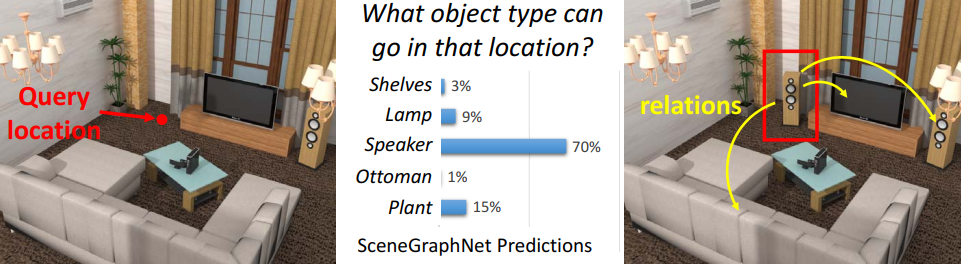
\includegraphics[width=0.8\linewidth]{fig_1.png}
  \caption{SceneGraphNet captures relationships between objects in an input 3D
    scene through iterative message passing in a dense graph to make object
    type predictions at query locations.}%
  \label{fig:1}
\end{figure}
%
Distribution is predicted through passing learned messages in a dense graph
whose \textbf{nodes} represent \textbf{objects} in the input scene and
\textbf{edges} represent spatial and structural \textbf{relationships}.


%%%%%%%%%%%%%%%%%%%%%%%%%%%%%%%%%%%%%%%%%%%%%%%%%%%%%%%%%%%%%%%%%%%%% Chapter 1
\section{Introduction}%
\label{sec:introduction}
The predicted distribution can be used in:
%
\begin{enumerate}
  \item Enhancing 3D object recognition in scenes by taking  into account the
    scene context (\Fig{2}).
  \item Automatically populating 3D scenes with more objects by evaluating the
    probability distribution at different locations in the scene (\Fig{3}).
  \item Providing object type recommendations to designers while modeling a 3D
    scene.
\end{enumerate}
%
\begin{figure}[htpb]
  \centering
  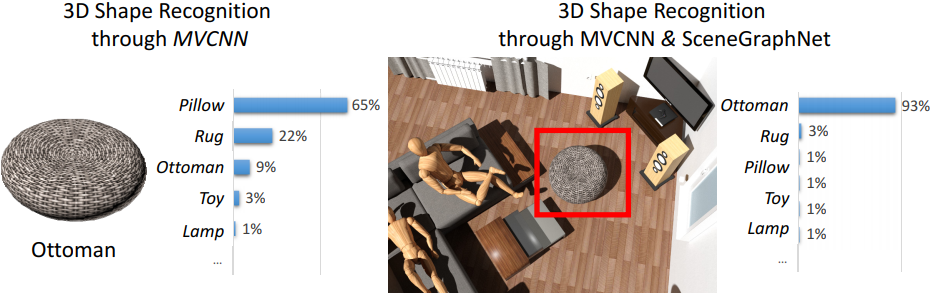
\includegraphics[width=0.8\linewidth]{fig_2.png}
  \caption{Context-based object recognition. Left: Object recognition using a
    multi-view CNN without considering the scene context. Right: Improved
    recognition by fusing the multi-view CNN and SceneGraphNet predictions
    based on scene context.}%
  \label{fig:2}
\end{figure}
%
\begin{figure}[htpb]
  \centering
  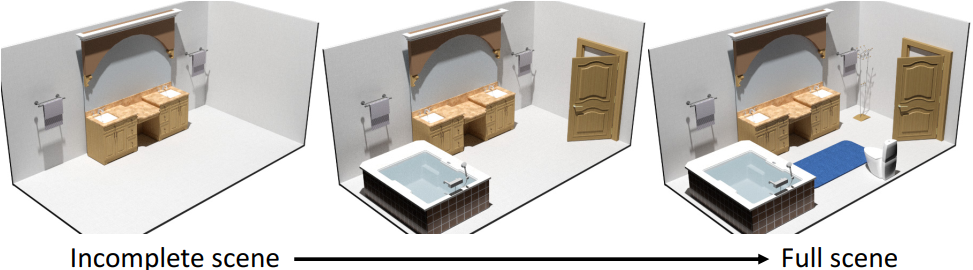
\includegraphics[width=0.8\linewidth]{fig_3.png}
  \caption{Iterative scene synthesis. Given an incomplete scene, our method is
    used to populate it progressively with more objects at their most likely
    locations predicted from SceneGraphNet.}%
  \label{fig:3}
\end{figure}

The method models the scene as a graph, where edges represent:
%
\begin{itemize}
  \item supporting
  \item surrounding
  \item adjacency
  \item co-occurrence
  \item long-range dependencies, \textit{e.g.}, the choice of a sofa in one
    side of a room can influence the selection of other sofas, chairs, or
    tables in the opposite side of the room to maintain a plausible object set
    and arrangement.
\end{itemize}
%
It is found that predictions are more plausible when not only local or strictly
hierarchical object relationships, but also long-range relationships are
modeled.

An attention mechanism is designed to weight different messages for predicting
objects at query locations.

Contributions:
%
\begin{itemize}
  \item a new graph neural network architecture to model short- and long-range
    relationships between objects in 3D indoor scene.
  \item an iterative message passing scheme, reinforced with an attention
    mechanism, to perform object-related prediction tasks in scenes, including
    spatial query answering, context-based object recognition, and iterative
    scene synthesis.
\end{itemize}

%%%%%%%%%%%%%%%%%%%%%%%%%%%%%%%%%%%%%%%%%%%%%%%%%%%%%%%%%%%%%%%%%%%%% Chapter 3
\section{Method}%
\label{sec:method}
In a scene $s$, given a query location $p$, the output is a probability
distribution over different object types/categories, $P(C \vert p, s)$
expressing how likely is for objects from each of these categories to fit well
in this location and match the scene context.
%
\begin{figure}[htpb]
  \centering
  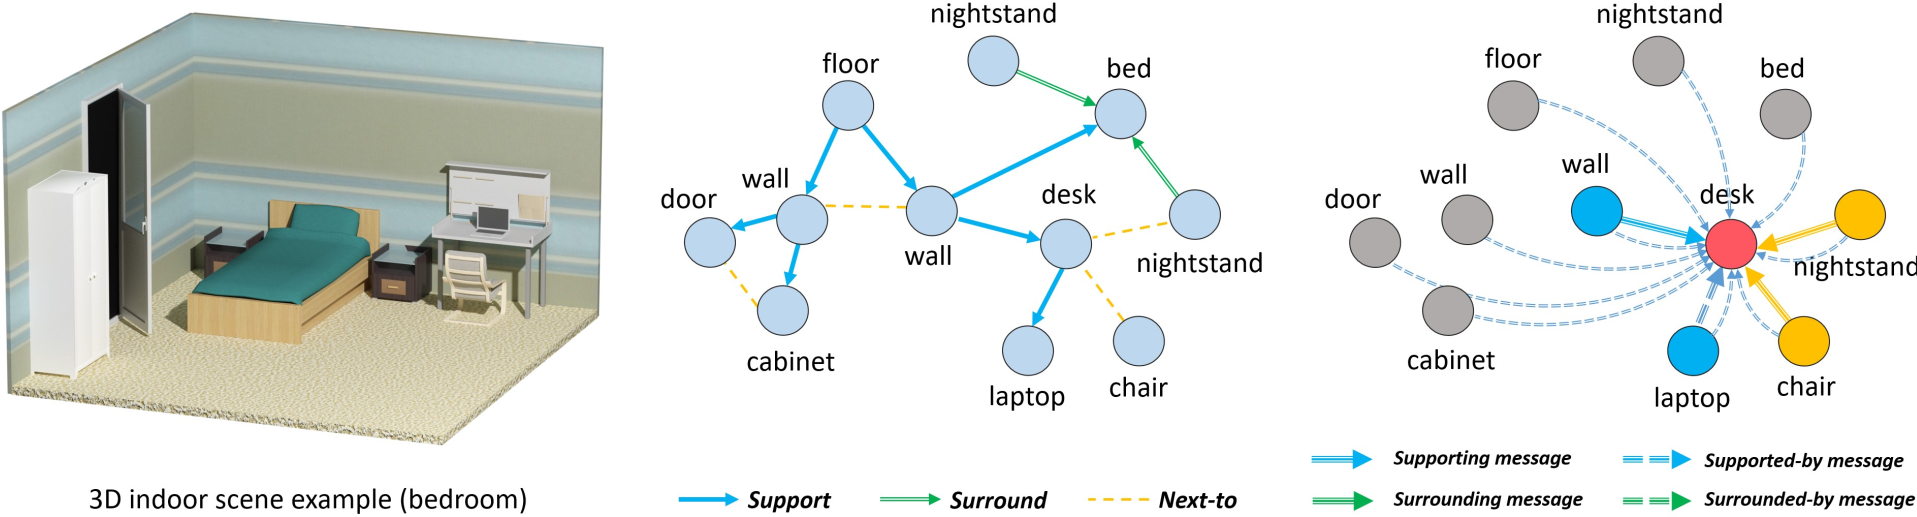
\includegraphics[width=0.8\linewidth]{fig_4.png}
  \caption{An example of the graph structure used for neural message passing in
    SceneGraphNet for a bedroom scene. Left: an input 3D scene. Middle: graph
    structure and object relationships we modeled (some relationships,
    \textit{e.g.} dense ``co-occurrence'' and ``next-to'' ones, are skipped for
    clarity). Right: messages received by the object ``desk'' from other nodes
    in the graph for all different types of relationships.}%
  \label{fig:4}
\end{figure}

%%%%%%%%%%%%%%%%%%%%%%%%%%%%%%%%%%%%%%%%%%%%%%%%%%%%%%%%%%%%%%%%%%% Chapter 3.1
\subsection{Message Passing}%
\label{sec:passing}
Each node carries a vectorial representation $h_i$ encoding information about
the shape and its scene context based on the message it receives from other
nodes. New messages are emitted from nodes; the message passing runs
iteratively.

The passing procedure:

\textbf{Initialization:} based on the shape representation $x_i$ at the node:
%
\begin{align}
  \label{eq:1}
  h^{(0)}_i = f_{init}(x_i; w_{init})
\end{align}
%
where $f_{init}$ is a two-layer MLP with learnable parameters $w_{init}$
outputting a 100-dimensional node representation. $x_i = [c_i, p_i, d_i]$
where $c_i$ is a one-hot vector representing category,
$p_i \in \mathcal{R^3}$ representing position, $d_i \in \mathcal{R^3}$
representing oriented bounding box lengths.

\textbf{Messages:} a message from node $k$ to $i$ carries information based on
$h^{(t)}_k$ and $h^{(t)}_i$ and the relationship $r$ between them.
%
\begin{align}
  \label{eq:2}
  m^{(r,t)}_{k \rightarrow i} = f^{r}_{msg}(h^{(t)}_k, h^{(t)}_i; w^{(r)}_{msg})
\end{align}
%
where $f^{r}_{msg}$ is a two-layer MLP with learnable parameters
$w^{(r)}_{msg}$ (weights are different per relationship $r$) outputting a
100-dimensional representation

\textbf{Weights on messages:} based on attention mechanism:
%
\begin{align}
  \label{eq:3}
  a_{k,i} = f_{att}(x_k, x_i; w_{att})
\end{align}
%
where $f_{att}$ is a two-layer MLP followed by a sigmoid layer with learnable
parameters $w_{att}$.

\begin{figure}[htpb]
  \centering
  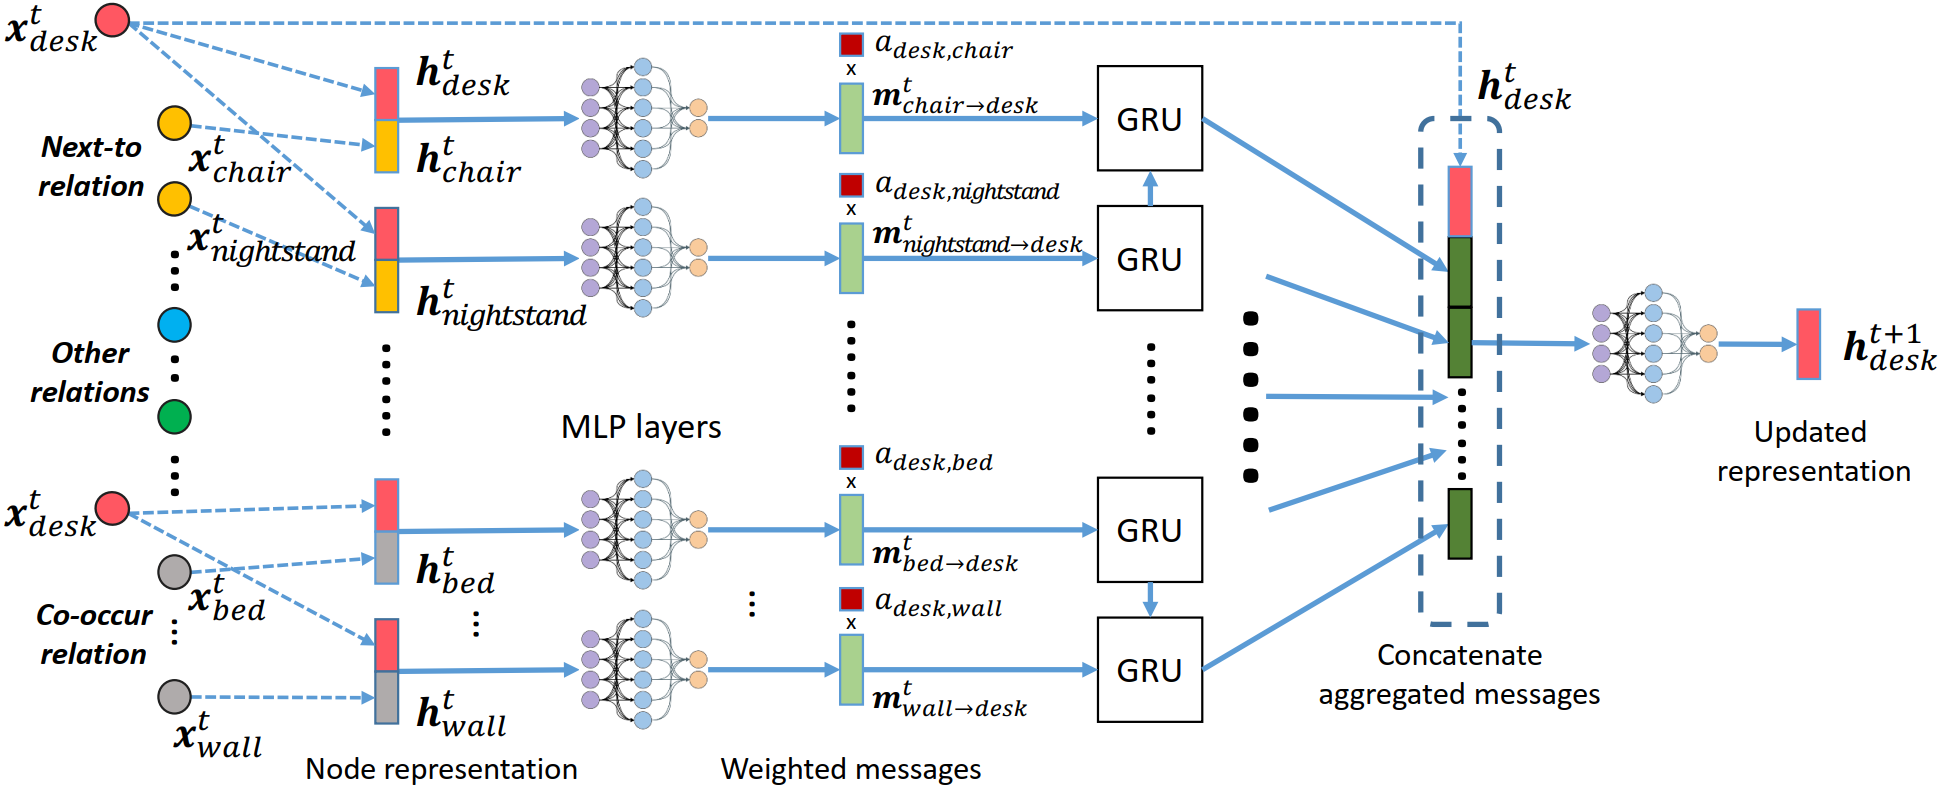
\includegraphics[width=0.8\linewidth]{fig_5.png}
  \caption{Overview of our message passing and underlying neural network
    architecture. We take the example in \Fig{4} to illustrate a single message
    passing iteration.}%
  \label{fig:5}
\end{figure}

%%%%%%%%%%%%%%%%%%%%%%%%%%%%%%%%%%%%%%%%%%%%%%%%%%%%%%%%%%%%%%%%%%%%% Chapter 6
\section{Experiments}%
\label{sec:experiments}
(Omitted.)


% \newpage
%%%%%%%%%%%%%%%%%%%%%%%%%%%%%%%%%%%%%%%%%%%%%%%%%%%%%%%%%%%%%%%%%%%%% Chapter 7
\section{Discussion}%
\label{sec:discussion}

\end{document}
